\documentclass[t]{beamer}
%\usetheme{Berlin}
\usetheme{Frankfurt}

\usepackage[english,spanish]{babel} 
\usepackage[utf8]{inputenc}         % Este paquete permite poner acentos directamente y e.es
\usepackage{multirow}
%\usepackage{ffbeamer}
%\usepackage{beamerthemem}

%%% Si la presentación es en ingles, de lo contrartio comentar %%%
%\chooselanguage{english}

\title[FFT]{FFT }
%\author[Nombre corto]{Kunst, James}
\date{\today}
%\date{August 2017}


\begin{document}

\begin{frame}
\maketitle
\end{frame}

%%%%%%%%%%%%%%%%%%%%%%%%%%%%%%%%
\section[Outline]{}
%%%%%%%%%%%%%%%%%%%%%%%%%%%%%%%%
\begin{frame}
       \frametitle{Contenido}	
        \vspace*{0.5cm}
       %\framesubtitle{Tabla de contenidos}	
       \tiny{\tableofcontents}
\end{frame}
%%%%%%%%%%%%%%%%%%%%%%%%%%%%%%%%%


%\begin{frame}
%\frametitle{Photonic assisted ADC}	
%\vspace*{0.5cm}
% \begin{figure}[ht]
%    \centering
%  \includegraphics[height=0.35\paperheight]{image/padc1.png}
% \includegraphics[height=0.4\paperheight]{image/padc2.png}
%    \end{figure}
%\end{frame}

\section{Enunciado}

\section{FFT 16 Puntos}

\section{}
\section{}

\section{}
\section{FFT 128 puntos}



\section{Versiones RTL y optimizacion}

\subsection{Version 1}
\begin{frame}
\frametitle{V1}	
%\vspace*{-0.8cm}
%%%%%%%%%%
\begin{columns}[T] % align columns
\begin{column}{.7\textwidth}
\vspace*{-0.9cm}
 \begin{figure}[ht]
    \centering
  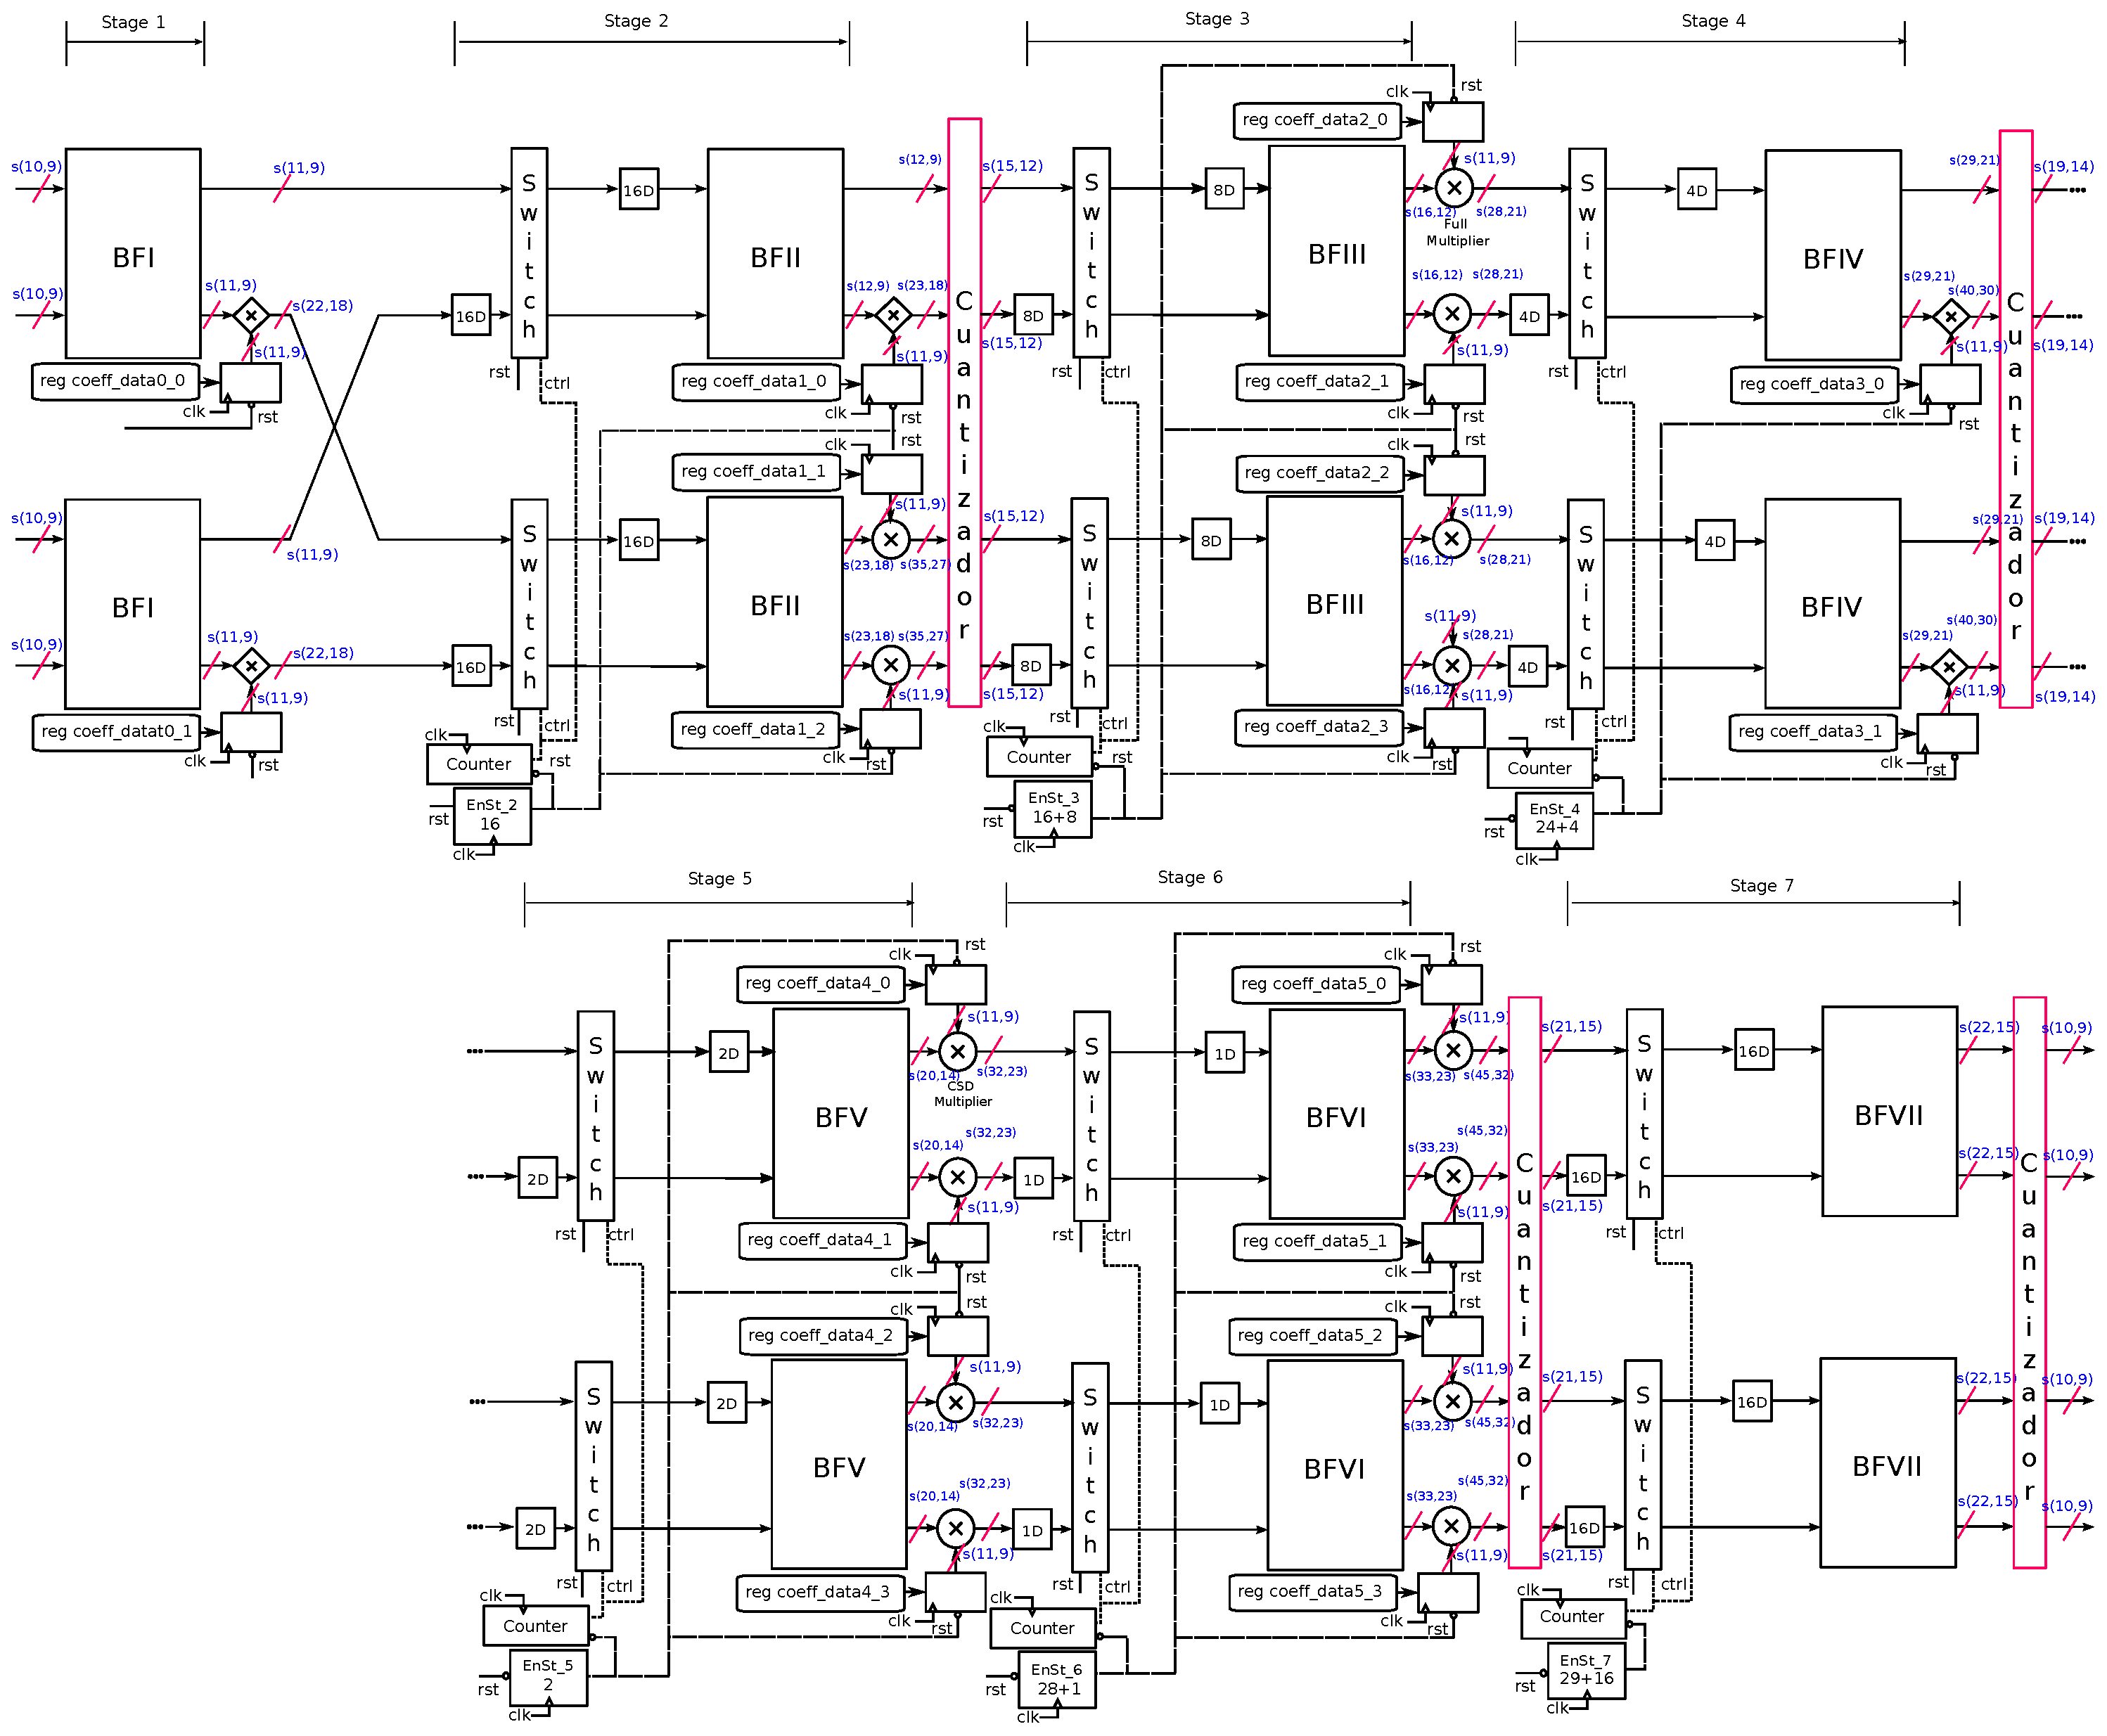
\includegraphics[height=0.72\paperheight]{image/V1_esquema_p.eps} \\
    \end{figure}

\end{column}%
%%%%%%%%%%

%%%%%%%%%%
\begin{column}{.3\textwidth}


\begin{itemize}
\item
\item
\item
\item
\item
\item
\item
\item
\item
\item
\end{itemize}

\end{column}
\end{columns}

\end{frame}

\subsection{Version 2}

\begin{frame}
\frametitle{V2}	
%\vspace*{-0.8cm}
%%%%%%%%%%
\begin{columns}[T] % align columns
\begin{column}{.7\textwidth}
\vspace*{-0.9cm}
 \begin{figure}[ht]
    \centering
  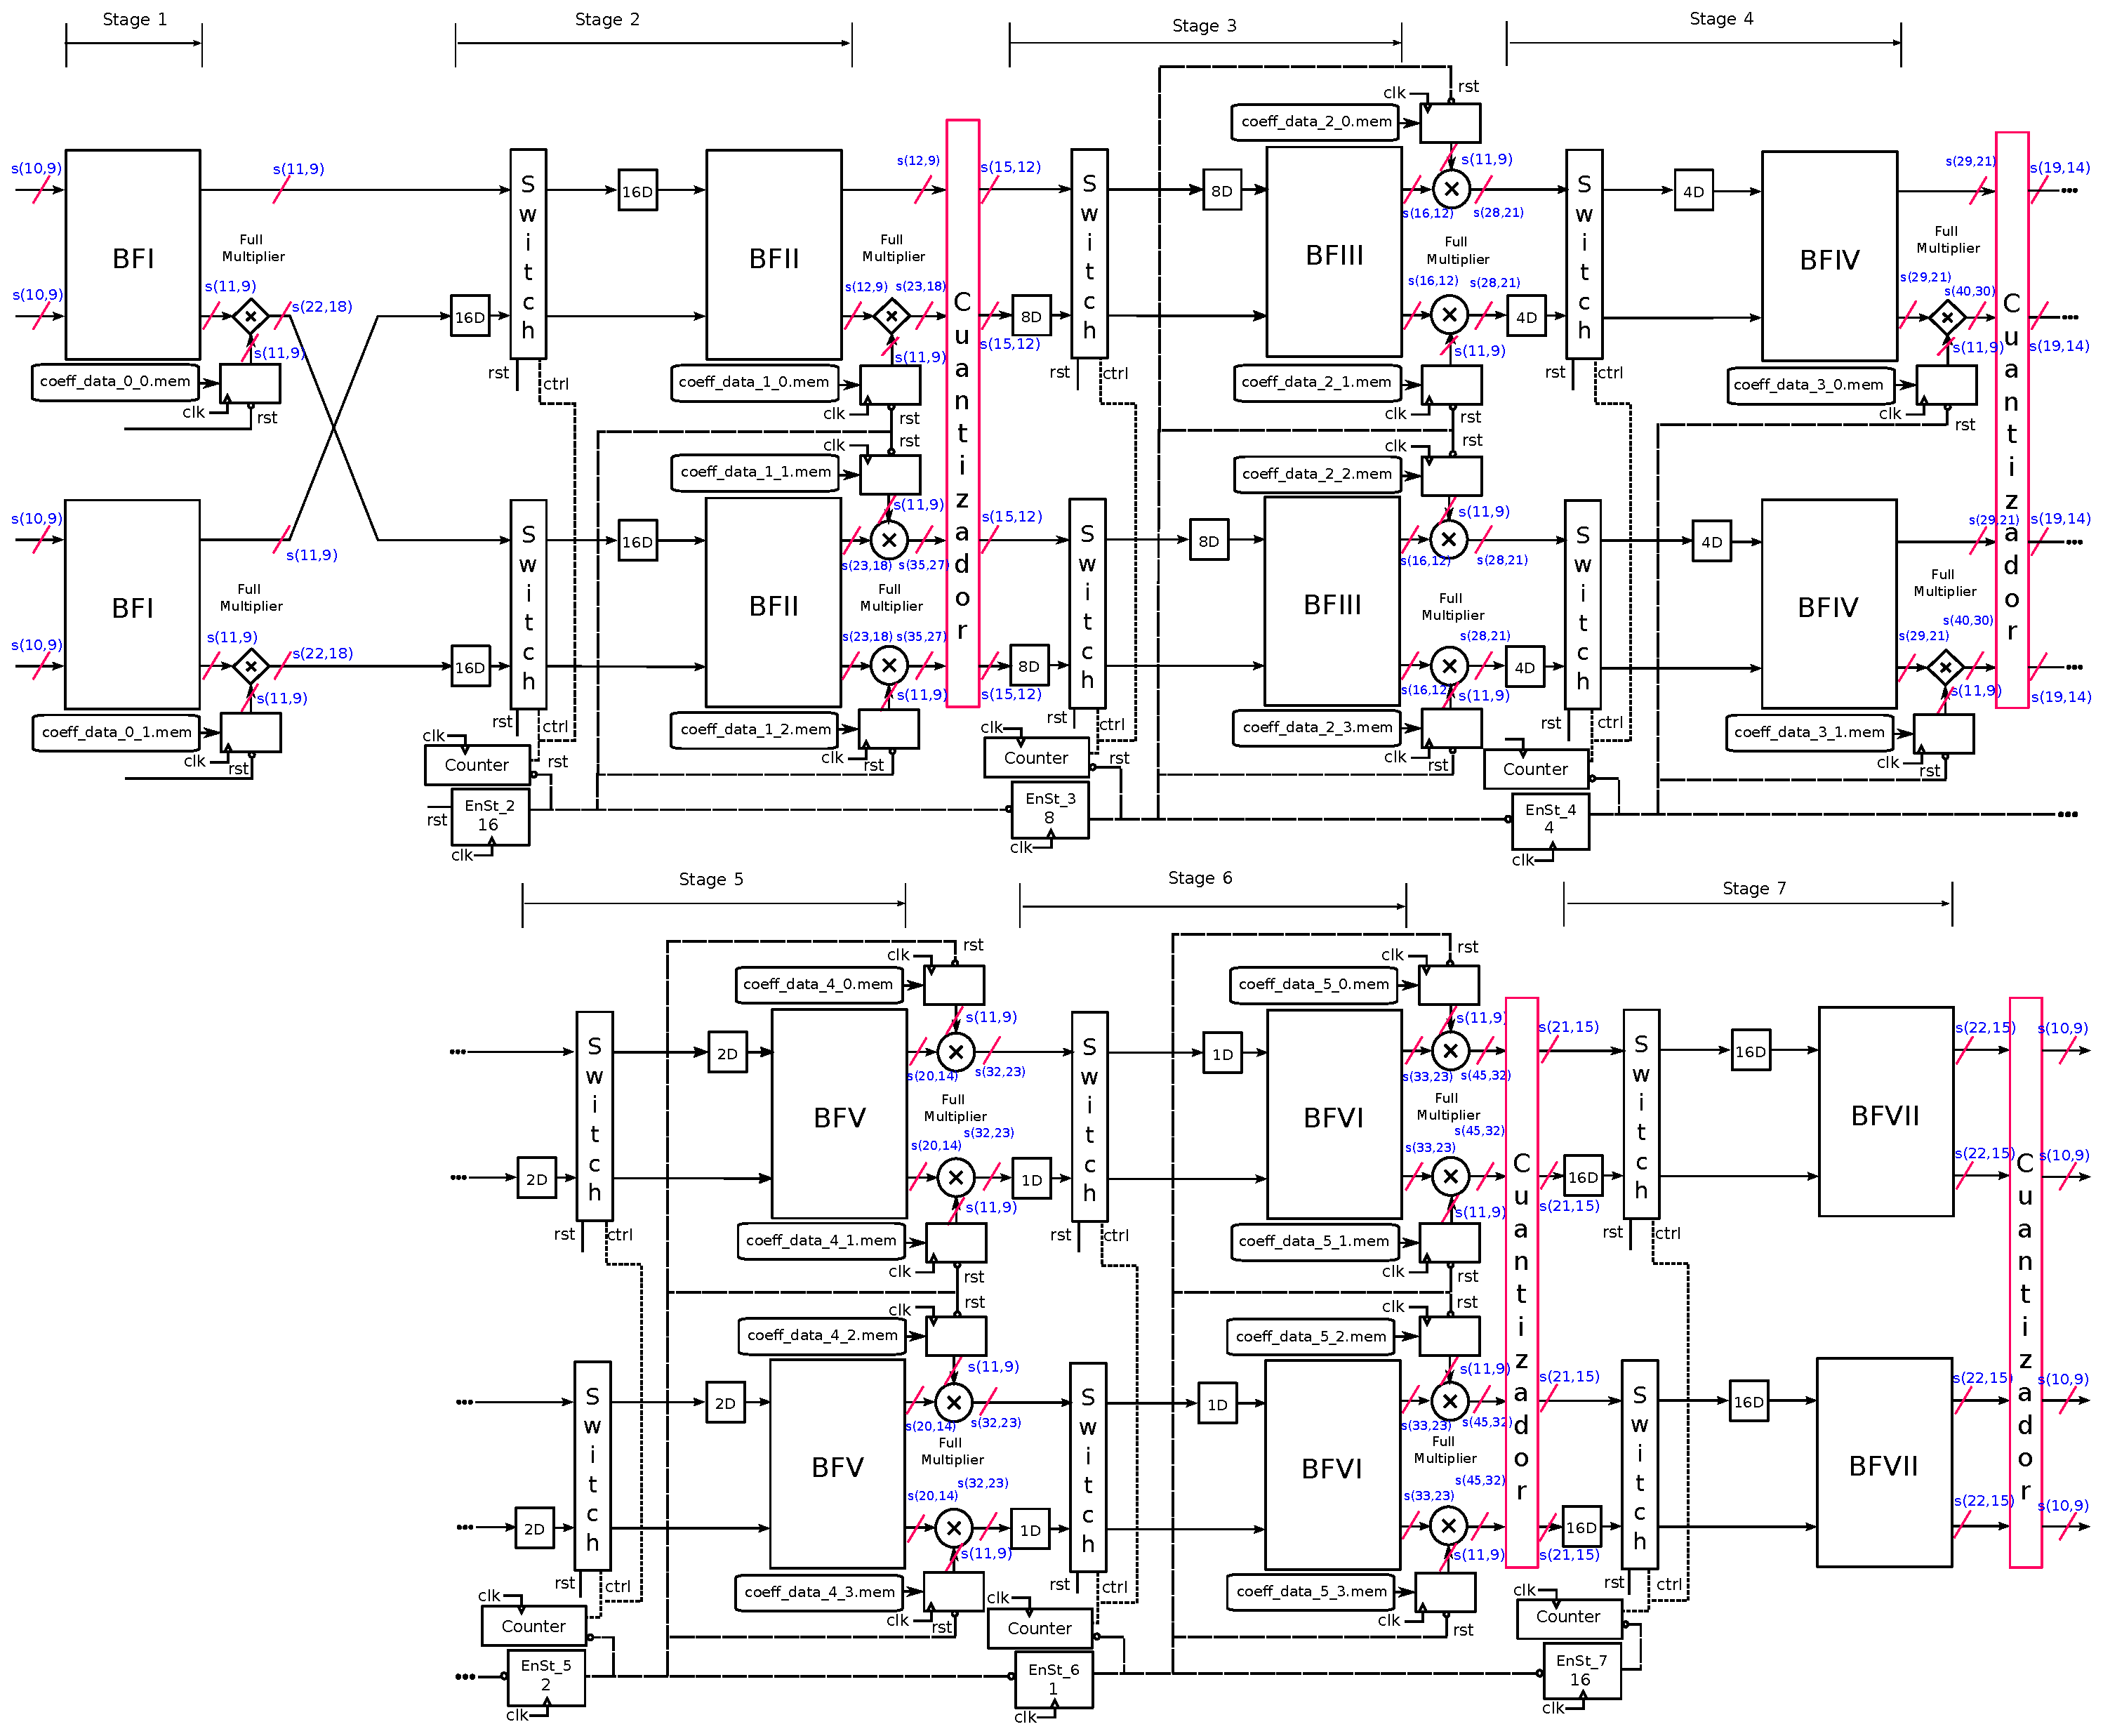
\includegraphics[height=0.72\paperheight]{image/V2_esquema_p.eps} \\
    \end{figure}

\end{column}%
%%%%%%%%%%

%%%%%%%%%%
\begin{column}{.3\textwidth}


\begin{itemize}
\item
\item
\item
\item
\item
\item
\item
\item
\item
\item
\end{itemize}

\end{column}
\end{columns}

\end{frame}

\subsection{Version 3}
\begin{frame}
\frametitle{V3}	
%\vspace*{-0.8cm}
%%%%%%%%%%
\begin{columns}[T] % align columns
\begin{column}{.7\textwidth}
\vspace*{-0.8cm}

 \begin{figure}[ht]
    \centering
  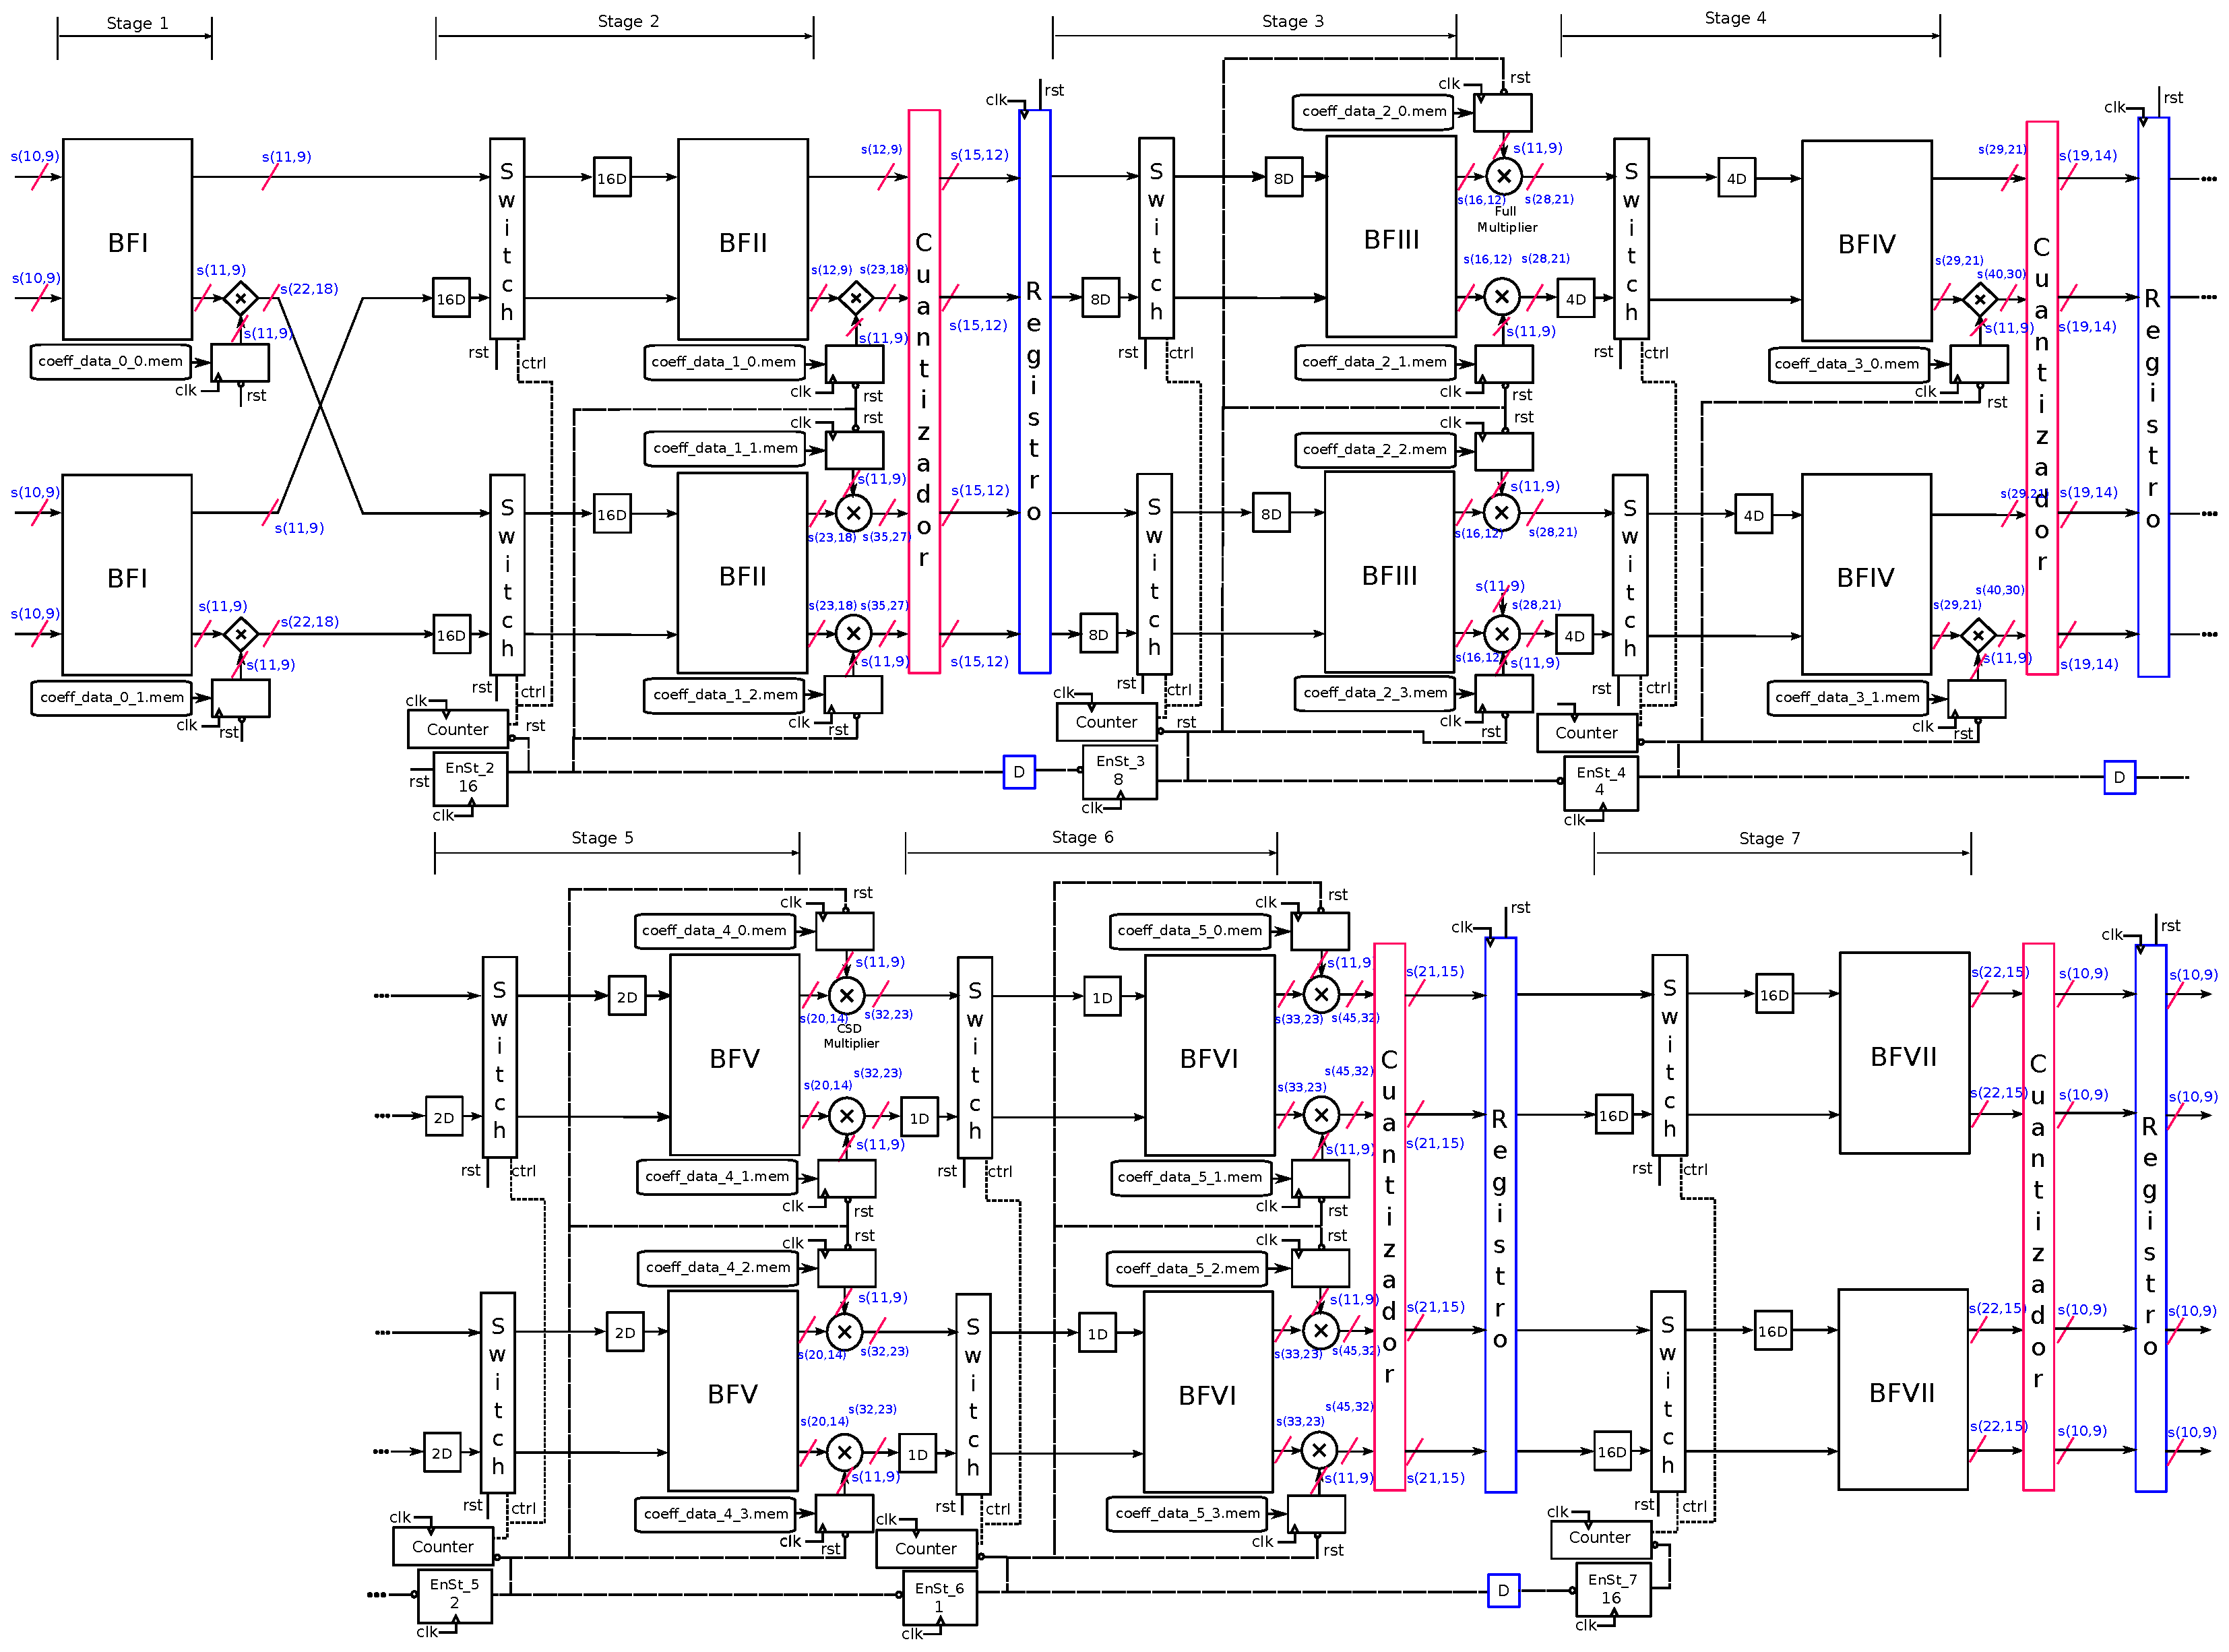
\includegraphics[height=0.66\paperheight]{image/V3_esquema_p.eps} \\
    \end{figure}

\end{column}%
%%%%%%%%%%

%%%%%%%%%%
\begin{column}{.3\textwidth}


\begin{itemize}
\item
\item
\item
\item
\item
\item
\item
\item
\item
\item
\end{itemize}

\end{column}
\end{columns}

\end{frame}



\subsection{Version 4}

\begin{frame}
\frametitle{V4}	
%\vspace*{-0.8cm}
%%%%%%%%%%
\begin{columns}[T] % align columns
\begin{column}{.7\textwidth}
\vspace*{-0.8cm}
 \begin{figure}[ht]
    \centering
  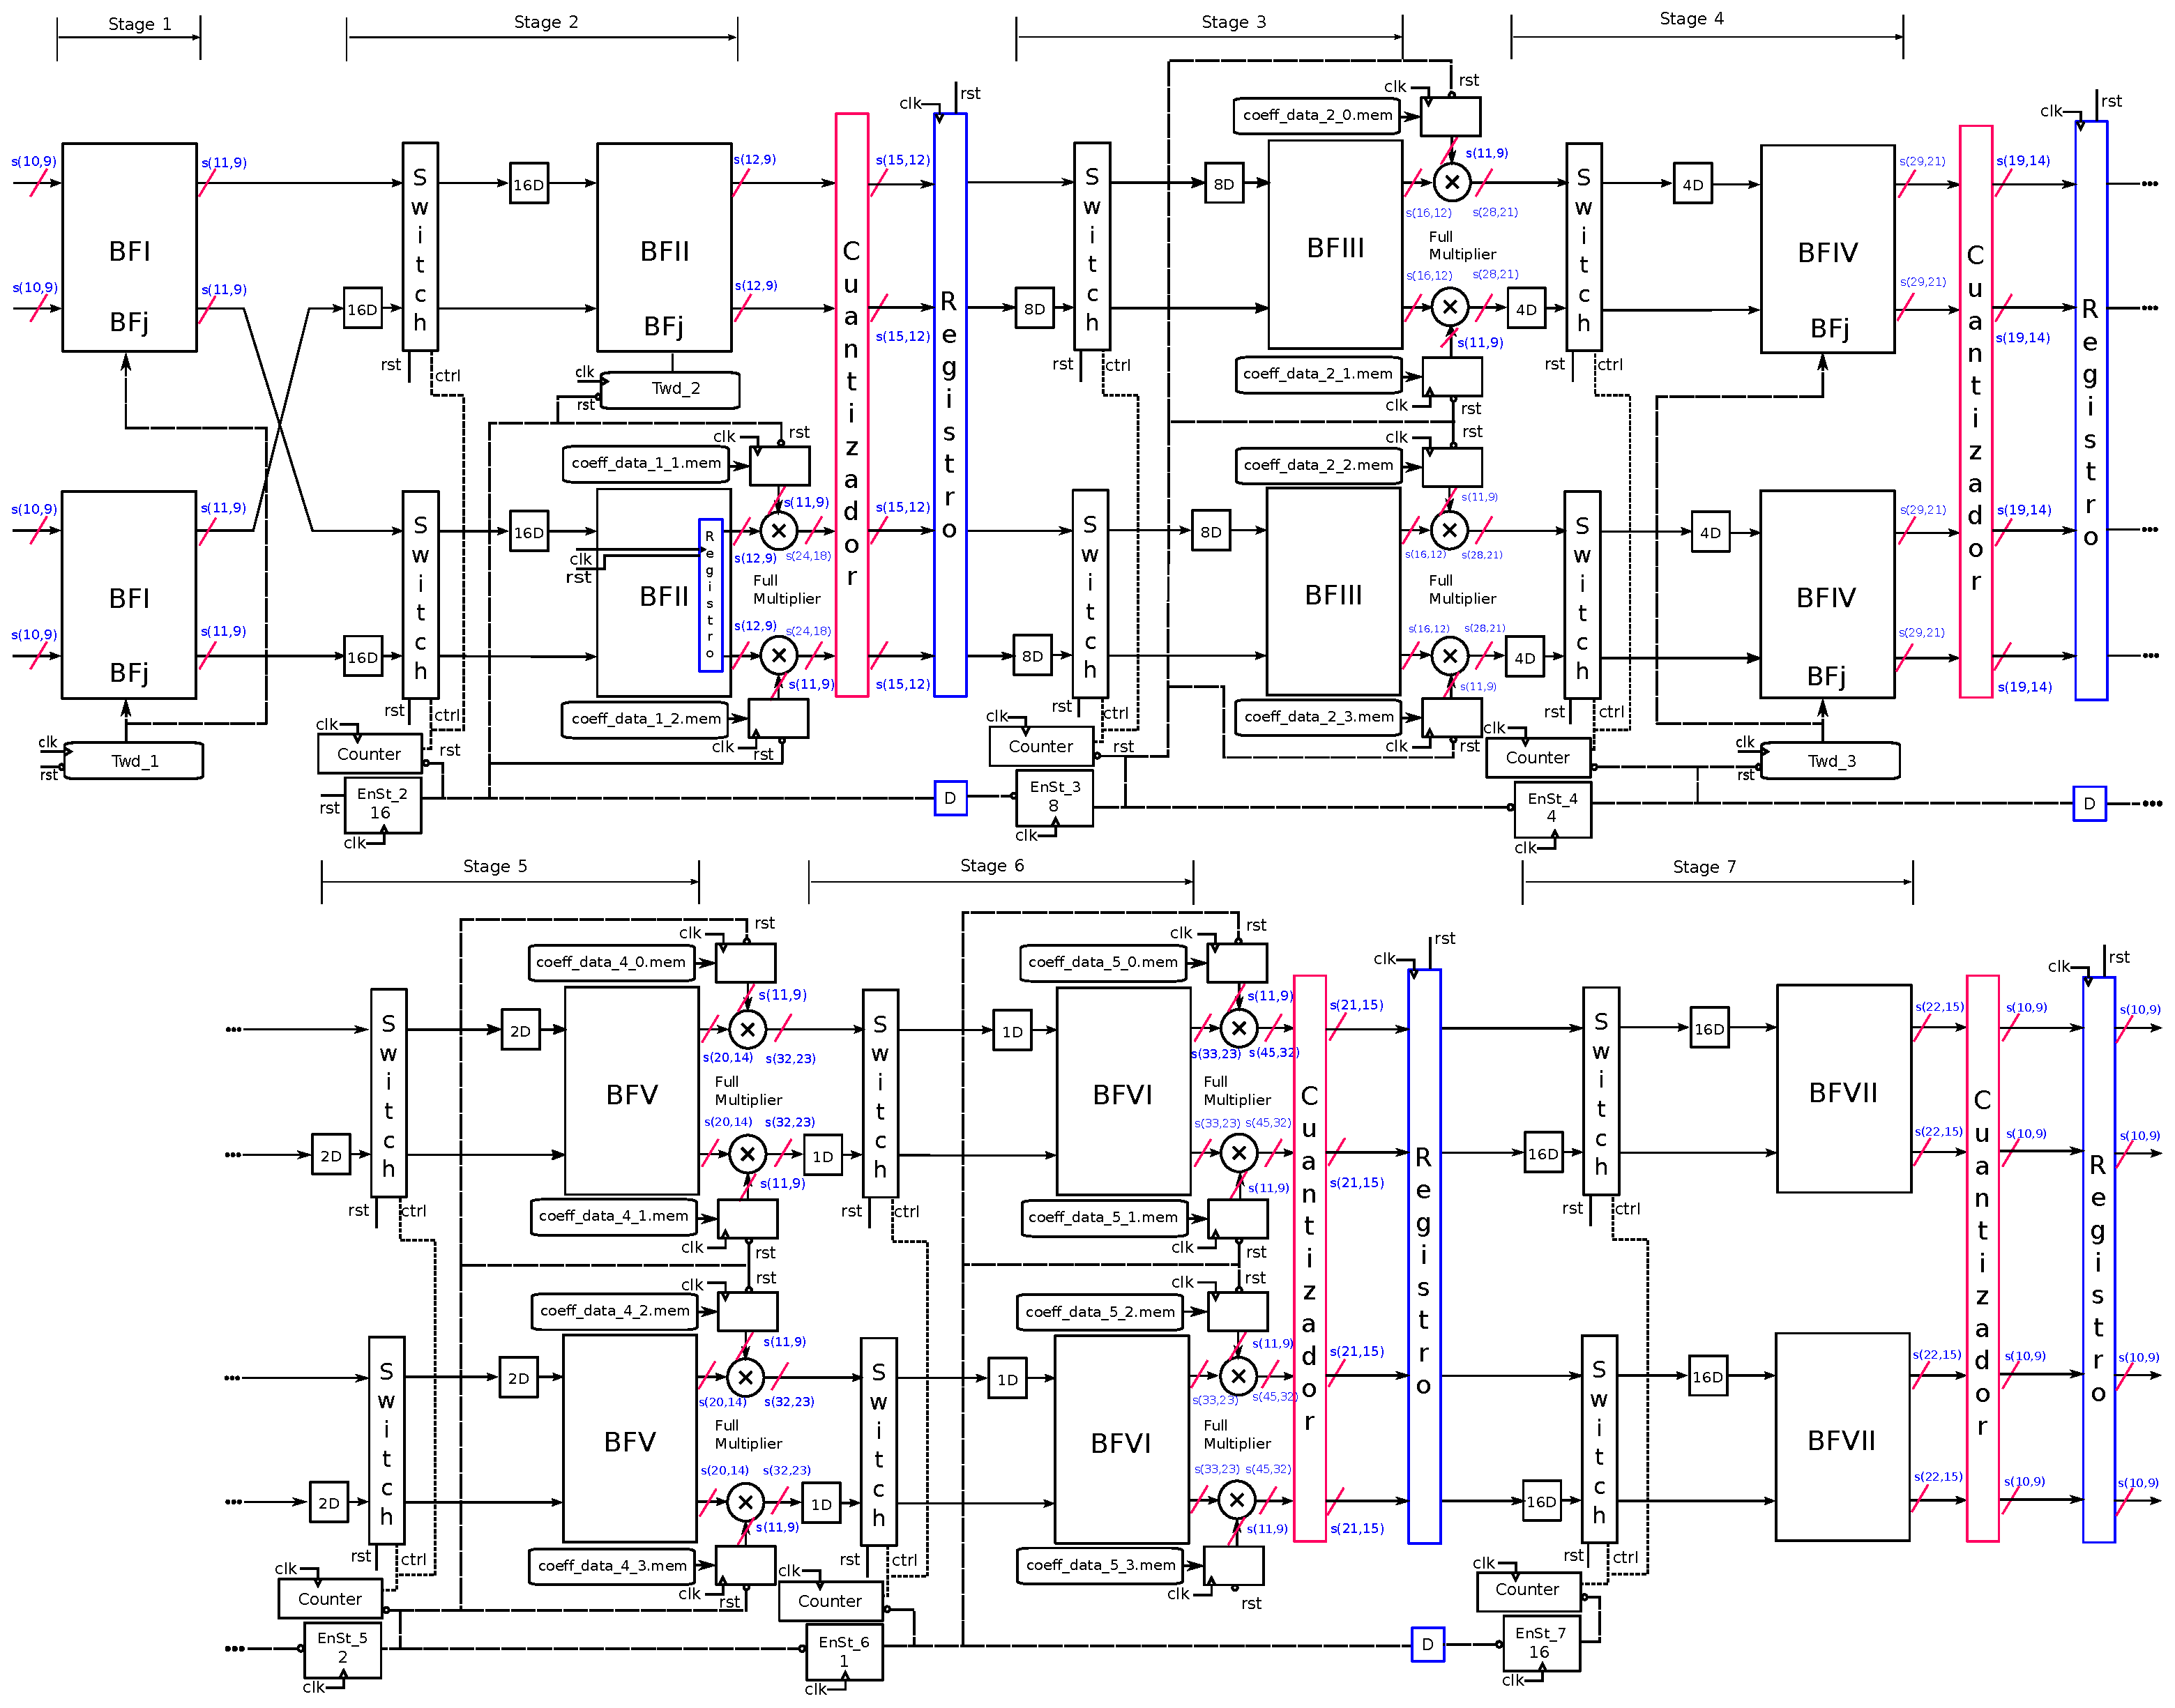
\includegraphics[height=0.7\paperheight]{image/V4_esquema_p.eps} \\
    \end{figure}

\end{column}%
%%%%%%%%%%

%%%%%%%%%%
\begin{column}{.3\textwidth}


\begin{itemize}
\item
\item
\item
\item
\item
\item
\item
\item
\item
\item
\end{itemize}

\end{column}
\end{columns}

\end{frame}

\subsection{Version 5}

\begin{frame}
\frametitle{V5}	
%\vspace*{-0.8cm}
%%%%%%%%%%
\begin{columns}[T] % align columns
\begin{column}{.7\textwidth}
\vspace*{-0.8cm}
 \begin{figure}[ht]
    \centering
  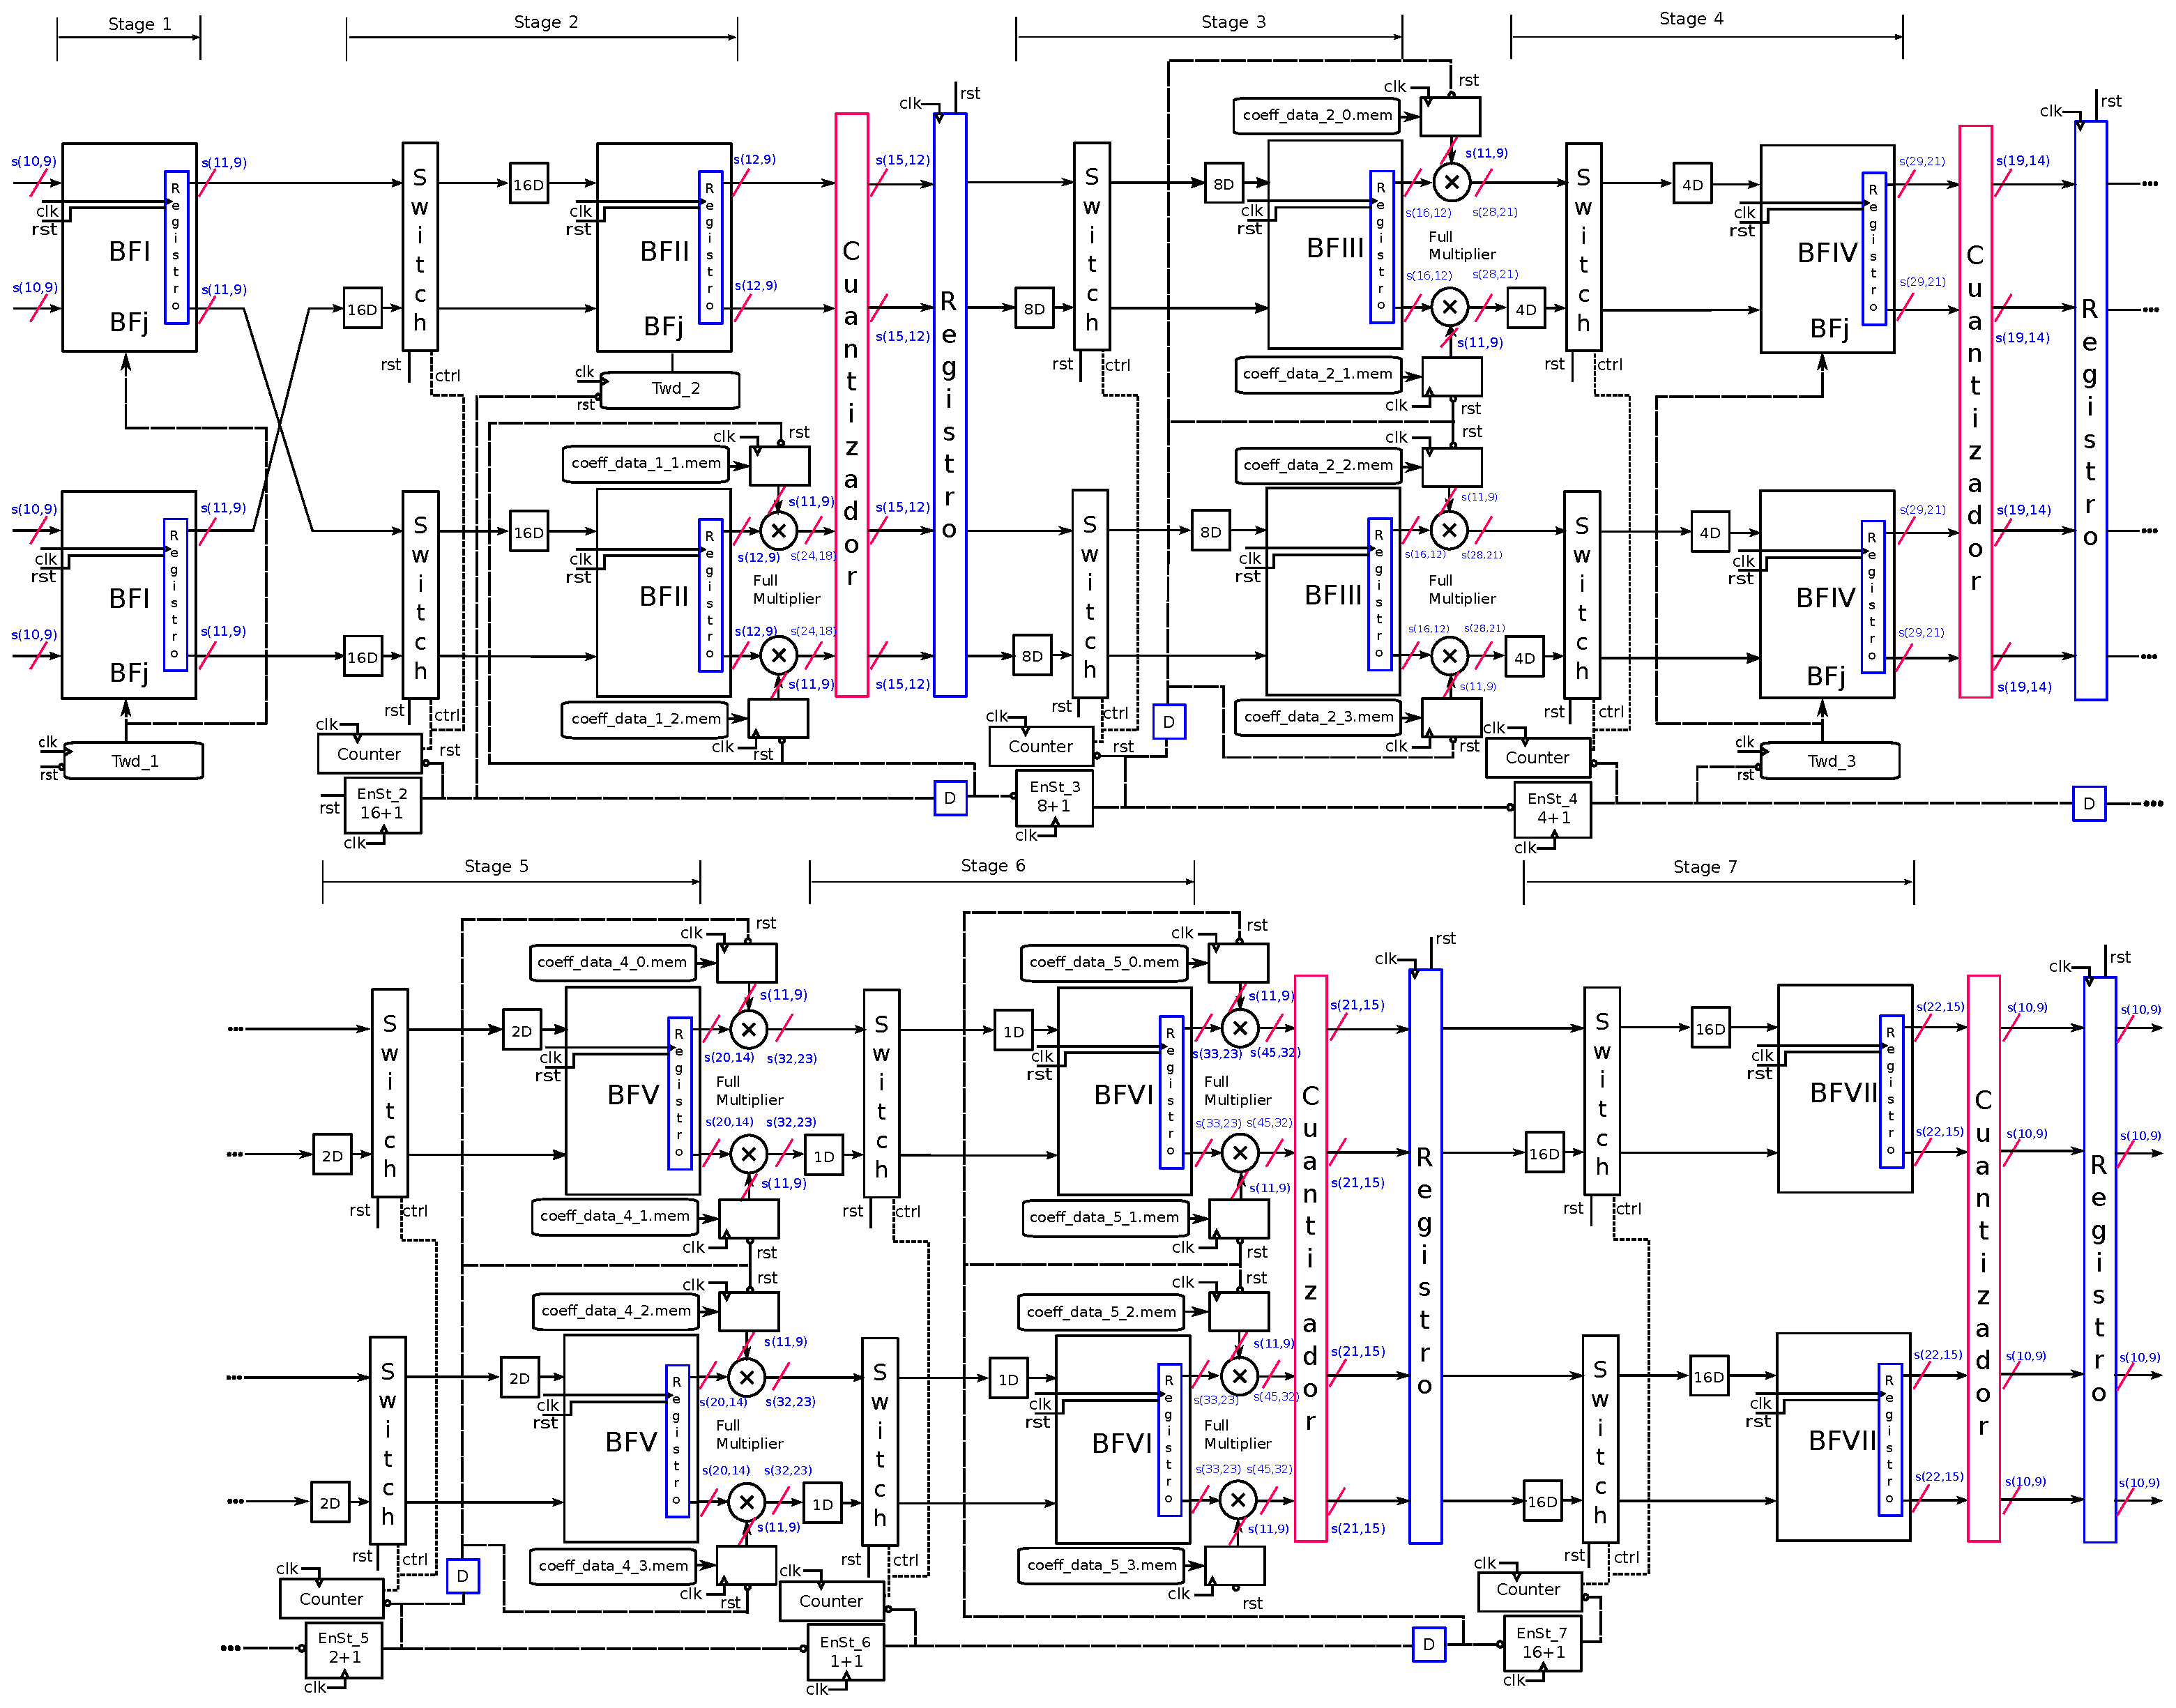
\includegraphics[height=0.7\paperheight]{image/V5_esquema_p.eps} \\
    \end{figure}

\end{column}%
%%%%%%%%%%

%%%%%%%%%%
\begin{column}{.3\textwidth}


\begin{itemize}
\item
\item
\item
\item
\item
\item
\item
\item
\item
\item
\end{itemize}

\end{column}
\end{columns}

\end{frame}

\subsection{Version 6}
\begin{frame}
\frametitle{V6}	
%\vspace*{-0.8cm}
%%%%%%%%%%
\begin{columns}[T] % align columns
\begin{column}{.7\textwidth}
\vspace*{-0.8cm}
 \begin{figure}[ht]
    \centering
  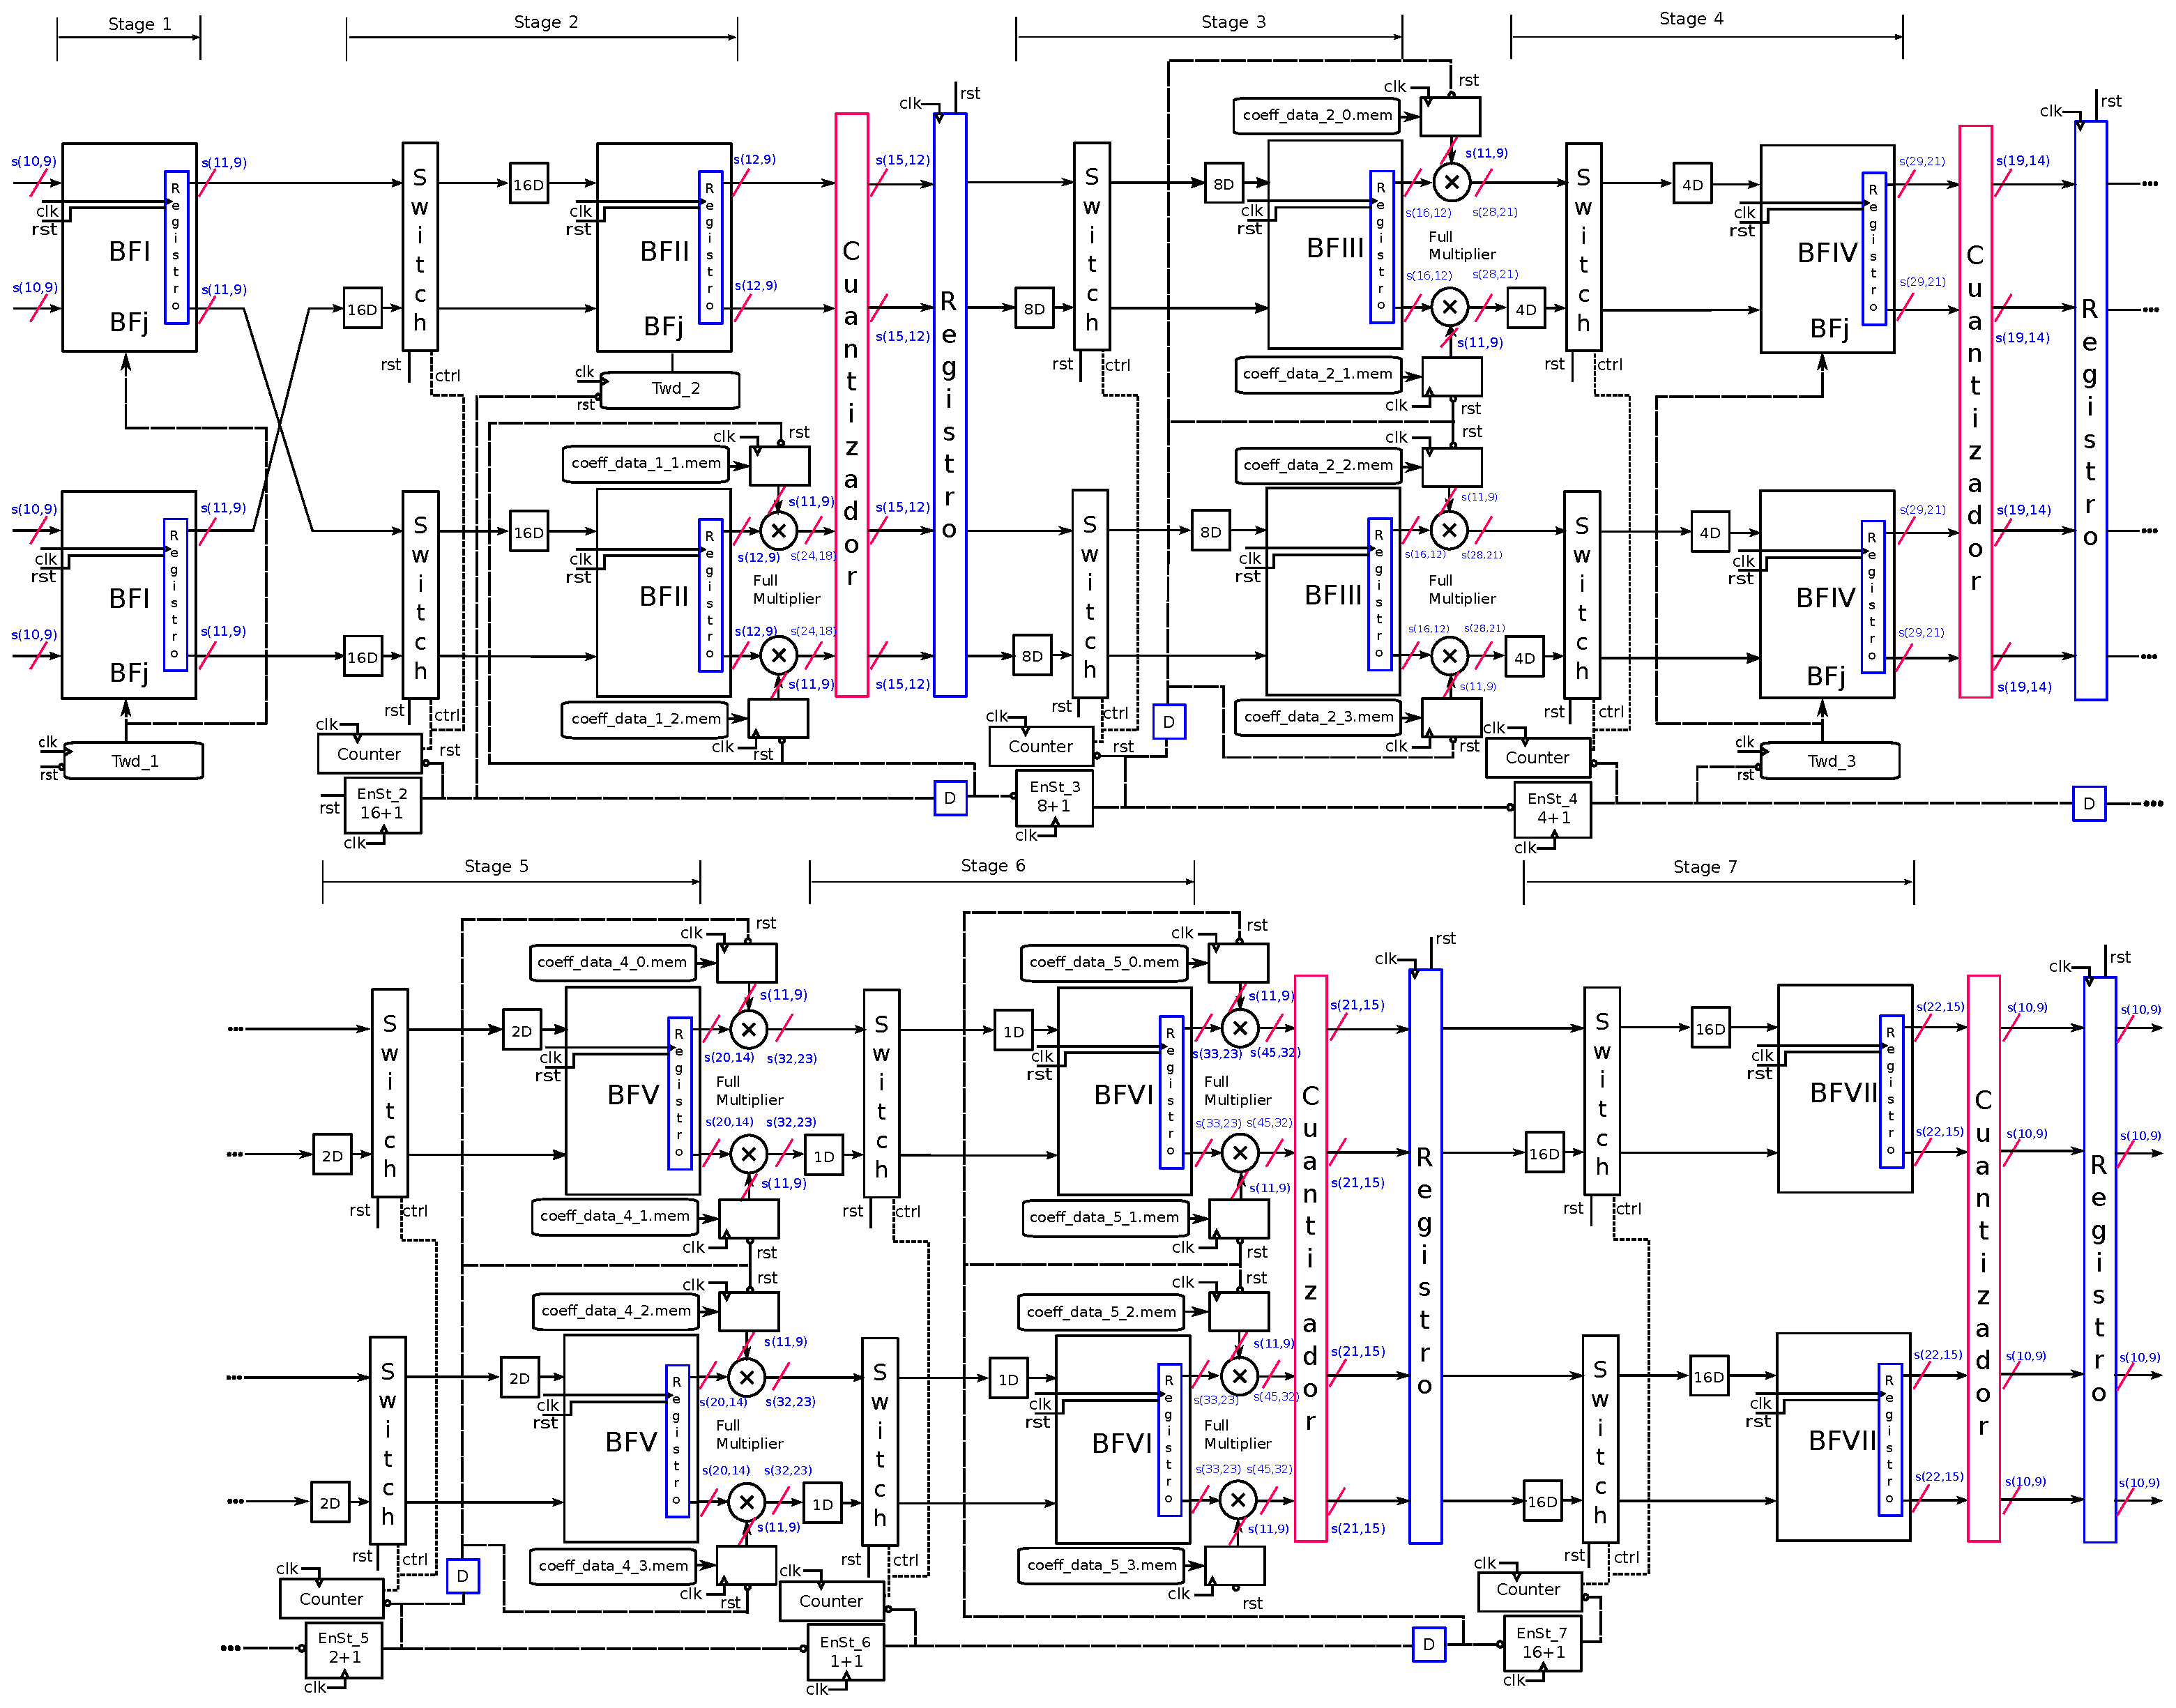
\includegraphics[height=0.7\paperheight]{image/V5_esquema_p.eps} \\
    \end{figure}

\end{column}%
%%%%%%%%%%

%%%%%%%%%%
\begin{column}{.3\textwidth}


\begin{itemize}
\item
\item
\item
\item
\item
\item
\item
\item
\item
\item
\end{itemize}

\end{column}
\end{columns}

\end{frame}

\section{Comparacion}

%%%%%%%%%%%%%%%%%%%%%%%%%%%%%%%%-----END-----%%%%%%%%%%%%%%%%%%
\begin{frame}
 \frametitle{Fin}
   %\framesubtitle{The end}
\vspace*{2cm}
\centering
\begin{Huge}
    ¡Gracias!
\end{Huge}
\end{frame}
\end{document}


%%%%%%%%%%%%%%%%%%%%%%%%%%%%%%%%%%%%%%%%%%%%%%%%%%%%%%%%%%%%%%%%%%%%%%%%%%%%%%%%%%%%%%%%%%%%%%%%%%%%%%%%%%%%%%%%%%%%%%%%%%%%%%%%%%%%%%%%%%%%%%%%%%%%%%%%%%%%%%%%%%%%%%%%%%%%%%%%%%%%%%%%%%%%%










